\documentclass[]{report}

\usepackage{minted}
% Margin settings
\usepackage[a4paper, portrait, margin=1in]{geometry}
%Table of Contents settings
\usepackage{hyperref}
\hypersetup{linktoc=all}
% Chapter settings
\usepackage{titlesec}
\titleformat{\chapter}[display]{\normalfont\Large\bfseries}{}{0.5ex}{}{}
% Paragraph settings
\setlength{\parskip}{1em}
\setlength{\parindent}{0pt}
\linespread{1.6} % Double line-spacing
% Images
\usepackage{graphicx}

% Title Page
\title{Chess for students; written in Python}
\author{Alexander Saoutkin}


\begin{document}
\maketitle
\pagenumbering{gobble}
\tableofcontents
\newpage
\chapter{Analysis}
\pagenumbering{arabic}
\section{Introduction}
The goal of this project was to build a desktop application which can be used to play chess amongst 2 human players. It will be used by those who attend chess club to not only play games but to save, load and continue playing them. This program is to be developed in Python and for the graphical user interface Qt has been chosen, with the Pyside library serving as a python wrapper around the Qt GUI framework. 

It consists of a visual representation of a chess board which is held in a table GUI element. This allows players to move pieces via clicking on a piece and then on the place it wants to move the piece to. It contains several buttons, which all complete several different functions. There is functionality to start a new game and to save, and load, existing games. Saving a game works by converting a python dictionary into JSON format and saving it in an existing JSON file by adding it to an array of dictionaries (games). If this file does not exist then the program allows the user to select a location for a new JSON file to be created, this location is saved as a setting so that the program can find this location again whenever it is relaunched.
 
Loading a game opens the JSON file from the location path that is saved as a setting and scans the array of games, showing them as a table in a dialog, so that the user can choose which game to open. If the location of the file does not exist, then the user is given the option of locating a different pre-existing JSON file to open from if it exists.

As already mentioned, the JSON file holds an array of games. A game contains the data needed to load a game: pieces and their positions, total moves, state of the game and other variables that are used to determine whether certain moves are possible, such as castling. Each game has a unique ID which allows users to load game that haven't been finished and to carry them on. For the program's loading and saving feature to be most useful for the school's chess club, it is best to store the JSON file in the school's shared area such that all games can be loaded and saved from any computer that has this program installed.

\section{Rules of Chess}
As with any game, there are rules that have to be adhered to for a valid game to be played. For me to have a viable solution to the problem identified, the program I create must follow the rules of chess. Thus in this section I will discuss what these rules are.
\subsection{The Game Board}
\begin{center}
	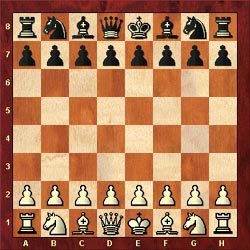
\includegraphics[width=0.4\textwidth]{images/boards/initial_board}
\end{center}
The initial starting position of the board contains all the types of pieces in the game: pawn, king, queen, bishop, knight and rook. From this point onwards, white is the first to move. Once white has completed a legal move it is then black's turn to do the same and the game continues until the game has reached the state of checkmate and stalemate, which will be explained in detail later. Only one piece can occupy a square on the board, thus a piece cannot take one of its own pieces but can capture opposing pieces as long as it isn't a king.

\paragraph{Note:}when the types of moves that a certain type of piece can make are discussed below, it is assumed that when moved, it does not put the player who is moving the piece into check. In addition, it will be assumed that the move does not mean that the moving piece is in the same place. If this is the case then the move is illegal.
\subsection{Pawns}
\begin{center}
	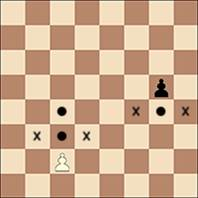
\includegraphics[width=0.3\textwidth]{images/boards/pawn_movement}
\end{center}
The pawn is a type of piece and has two types of moves, depending on the situation. If the pawn is in the same space as its starting position then it can either move one or two spaces forward, given that there is no piece in the way of this movement. In any other position it is only able to move into the next square forward, as long as there is no other piece currently there. 
\subsubsection{Promotion}
\begin{center}
	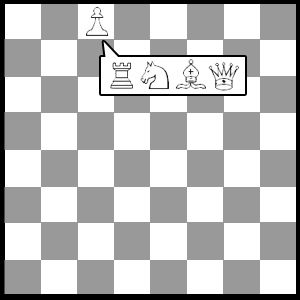
\includegraphics[width=0.3\textwidth]{images/boards/promotion}
\end{center}
When a pawn reaches the other side of the board the pawn must be changed to an additional piece that is a rook, knight, bishop or queen.
\subsubsection{En Passant}
\begin{center}
	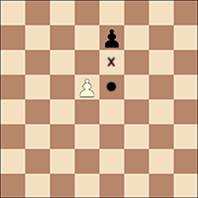
\includegraphics[width=0.3\textwidth]{images/boards/en_passant}
\end{center}
As can be seen above, if a pawn is moved two spaces forward such that it is horizontally adjacent to an opposing pawn once it is moved, the opposing pawn has an opportunity to capture the pawn and move to the ‘x' marked on the diagram. When this opportunity occurs, whether it is taken or not, it cannot be done again by that player for the rest of the game.
\subsection{Kings}
\begin{center}
	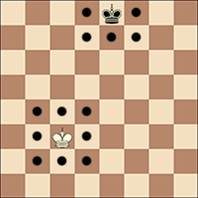
\includegraphics[width=0.3\textwidth]{images/boards/king_movement}
\end{center}
The king can move to any adjacent square provided that it is not in check once it completes the move. In addition it should not be adjacent diagonally, horizontally or vertically, to the opposing king after it has moved. 
\subsubsection{Castling}
\begin{center}
	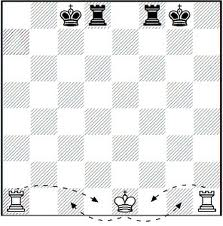
\includegraphics[width=0.3\textwidth]{images/boards/castling}
\end{center}
Castling is a move (shown above) that can be performed only if the king and rook have not been moved before. For castling to be performed no pieces must be in the way of the king and the rook moving and any of the squares in between them must not be attacked by an opposing piece.
\subsection{Bishop}
\begin{center}
	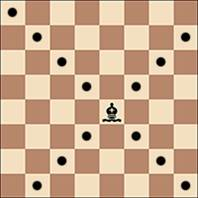
\includegraphics[width=0.3\textwidth]{images/boards/bishop_movement}
\end{center}
The bishop can move diagonally in any direction. Thus, it can only move on the colour of squares that are the same as its starting position.	
\subsection{Rook}
\begin{center}
	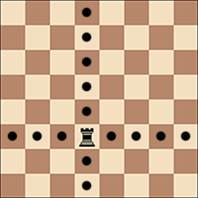
\includegraphics[width=0.3\textwidth]{images/boards/rook_movement}
\end{center}
The rook can move both vertically and horizontally in any direction.
\subsection{Queen}
\begin{center}
	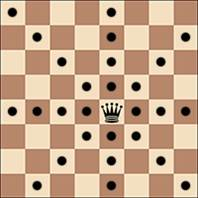
\includegraphics[width=0.3\textwidth]{images/boards/queen_movement}
\end{center}
The queen can both move anywhere diagonally, horizontally and vertically. In other words, a queen can be considered a combination of both the rook and the bishop.
\subsection{Knight}
\begin{center}
	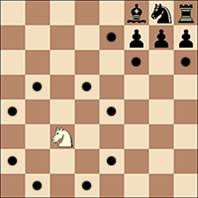
\includegraphics[width=0.3\textwidth]{images/boards/knight_movement}
\end{center}
The knight has one of the more interesting moving patterns. It can move in what is known as an L-shape. To be more precise, the possible moves of a knight can be calculated by moving 2 along vertically and then 1 horizontally either side, and vice-versa. Its attacking moves do not include the path to its possible moves.
\subsection{Game States}
In chess there are 3 types of game states that differ from normal play and restrict what legal moves can be made. Two of those are permanent (end of game) states: checkmate and stalemate. The other is check and this means that only moves that take a player out of check can be made. 
\subsubsection{Check}
\begin{center}
	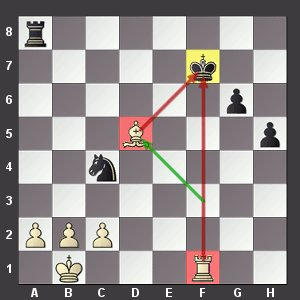
\includegraphics[width=0.3\textwidth]{images/boards/check_example}
\end{center}
Check occurs when a piece moves such that it is attacking the opposing king. An attacking move is such that if we theoretically suppose that the king is a piece that can be captured by a piece, then it would be captured if the piece moved there. An example of this is the image seen above. An important note is that for pawns this means they cannot check a king if it is horizontally ahead of it, as a pawn cannot move there if we theoretically supposed that a king is able to be captured. However, it can if the king is diagonally adjacent in front of the pawn. 
\subsubsection{Checkmate}
\begin{center}
	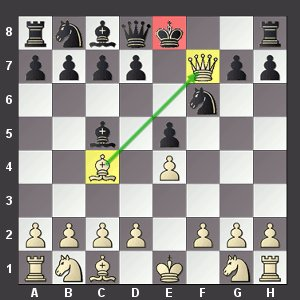
\includegraphics[width=0.3\textwidth]{images/boards/checkmate_example}
\end{center}
Checkmate occurs when a player is put into check and cannot make a move that brings themselves out of check. The person who is in check is the loser of the game and thus the opposing player is the winner. A well-known example is the scholar's mate which can be seen above. The queen cannot be taken by any piece and the king has nowhere to move without still being in check. In addition, the king cannot take the queen as it will put itself in check to the bishop. Thus black concedes the game as it is in a state of checkmate.
\subsubsection{Stalemate}
\begin{center}
	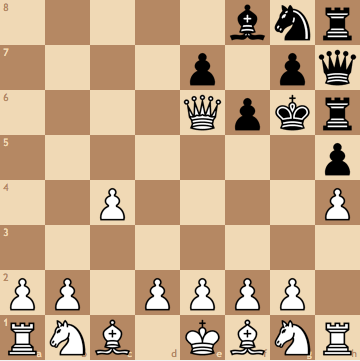
\includegraphics[width=0.3\textwidth]{images/boards/stalemate_example}
\end{center}
Stalemate occurs when a player who is not in check cannot make any legal moves and thus the game cannot continue. Above is an example of a stalemate. It is black's turn to move but it has no legal moves to make. Any movements are either not available to make or expose the king to being in check to either the far-right pawn or the queen. When a stalemate occurs the game is declared as drawn and there are no winners or losers.
\section{Setting}
The program was designed for the school's Chess club and is open for students from year 7 to 13. Chess club currently runs weekly at lunchtimes and is run by a physics teacher – Dr De Silva. Every year a primarily student run inter-house chess competition, with each house having a team of avid chess players, takes place to determine which house has the best chess players. As a member of chess club I identified and researched problems with the current system that the club uses. I also consulted with Dr De Silva about any problems that he has noted in the current system and have used this information to aid me in determining the objectives that I plan for the new system to implement.
\section{Users}
The primary users are those students who partake in the chess club and actively play chess amongst one another. It can also be used by the teacher that runs the club to record the results of games, which is paramount when there are competitions taking place. There is an additional benefit in that it can be played at any time and on any computer in the school area that has the program installed. This may be of good use to those who would like to play chess but are unable to go to the club due to other extra-curricular activities.
\section{System}
Currently most games that are played are not recorded because most are for recreational entertainment and so the result of the game is inconsequential, though results may be remembered by students and also may help in choosing players for the inter-house chess competition. Currently, when the inter-house chess competition happens the whiteboard in the classroom is used to show players who they are playing against and when the game is finished the result is written to the right of the matchings. Then the results are transferred to paper and are stored by the teacher who runs the club.
\section{Input}
All the results of games to do with a competition are recorded in a notebook and of course the movement of pieces is recorded on the board. All other games are not recorded at all and the location of pieces when a game is finished are generally not stored unless a student chooses to take a picture of the board.
\section{Processing}
Processing in the current system is fairly simple. Once a player has chosen where to move a piece, they pick it up and move it to the appropriate position on the board. If it is illegal it is assumed that the opponent will notice as it is in their best interest to not allow such a move. If that is the case then the piece is simply moved back to its place. The player who moves a piece also notes mentally if the piece that they have moved has resulted in a change in the state of the game.
\section{Output}
Output is simply where the player moves their piece on the board, which is visible to both players and any people watching. In addition, when a player moves a piece which results in the changing of the game state they must state this change openly to the opposing player.
\section{Problems with the Current System}
The current system consists of chess boards with pieces and paper if results want to be recorded. The main problem that was noticed was that as the club was only hosted on a single lunchtime a week, many games overran past lunchtime and so had to be stopped with no clear winner as the game had not finished. As the game was played on a physical board with pieces and the room that was used for the club is used for lessons as well, the current state of the game is not saved which resulted in the game effectively being cut short. This is incredibly frustrating, especially for higher-level players as their games tend to take longer to finish. 

Another problem came from when in-school chess competitions occurred. These competitions required results to be recorded such that it could be determined who plays who in further rounds of the competition, i.e. what teams play against one another in the final. These are recorded at lunchtime on the board and then recorded later on paper. There are of course problems with such a system. Firstly, results can easily be lost as it is held in one location. This also means that only one person can view the results at the time, unless the results are published in an e-mail which takes time to produce. In addition, it does not store the final state of the game when finished which may be of interest to students and teachers alike.

A problem that has been noted by students is that even though they are willing to attend chess club, many are unable to attend at lunchtimes on a certain day because they have other commitments and so end up not attending at all despite their desire to do so. Many students would like to be able to play chess games outside of club hours amongst each other with results recorded at school.
\section{Objectives}
After the analysis of the current system and the requirements that would be needed for an improved system I have created SMART (Specific, Measurable, Achievable, Realistic and Timely) objectives which make clear to me - the developer – what the client requires for their new system which has been determined to be accomplishable and adheres to all of the letters of the SMART abbreviation: Specific, Measurable, Achievable, Realistic, Timely.

The objectives of the new system are as follows:
\begin{enumerate}
	\item The showing of an interactive chess board allowing movement of pieces by users which adheres to all chess rules.
	\begin{enumerate}
		\item When program loads, show default chess starting position (a new game).
		\item Ensure only pieces of the moving player's corresponding colour are clickable.
		\item When a piece is clicked calculate all of its legal moves.
		\begin{enumerate}
			\item For each type of piece calculate where it could possibly go assuming there are no other pieces on the board (i.e. bishops diagonally, rooks horizontally/vertically etc.).
			\item Taking into account where other pieces are on the board, calculate the possible moves for that piece.
			\item Considering the moves that have been calculated, check that each position does not result in the moving player to be in check. 
			\begin{enumerate}
				\item If a move results in a player going into check then remove that move from the list of legal moves.
			\end{enumerate}
			\item When this calculation is done, cells in the table corresponding to the legal moves must be made clickable so that the player can move the appropriate piece there if they wish.
			
		\end{enumerate}
		\item After a piece is moved perform a check of the game state. If the state has changed (i.e. if a player has been put into check or the game has ended) then inform the user of this via a dialog.
		\item If the pawn has successfully reached the other side of the board, then open a dialog to let the user decide to what piece the pawn should be converted to.
	\end{enumerate}
	\item Allow the editing of player's names via textboxes.
	\item Allow a game that is currently in play to be saved.
	\begin{enumerate}
		\item If there is no file path to save the game to, prompt the user for a path and filename to save a new JSON file to.
		\item If there is a file path and the JSON file is found, then save the game to the file.
		\item If there is a file path and the JSON isn't found, then prompt the user for a path and filename to save a new JSON file to.
		\item If a game has been successfully saved, convey this information to the user via a dialog.
		\item If the player names have not been filled in, then do not save the game and inform the user that they have to fill in the names in the form of a dialog.
		\item If the game has an ID then save it by replacing the element of the games array with the same name by searching for the appropriate ID with a binary search.
	\end{enumerate}
	\item Allow a user to load a game and to continue to play it.
	\begin{enumerate}
		\item If the JSON file is not found then prompt the user to input the path to the game.
		\item Display the list of games in a table to allow the user to know which game to choose.
		\begin{enumerate}
			\item Information that must be shown in the table: ID, name of player 1 and 2, winner, moves made, last played.
			\item Using a quicksort algorithm, allow the user to sort the list of games based on parameters such as ID and the names of players.
		\end{enumerate}
	\end{enumerate}
\end{enumerate}
\chapter{Design}
\section{Overall System Design}
\subsection{Input}
The first type of input is selecting a piece on the board by clicking on a cell in the 8*8 table that contains a piece corresponding to the player's colour. At this point processing occurs and moves that are legal are added as cells that can be clicked on the table. After this, if a cell is clicked that is not a player's piece then the last clicked piece is moved to that location. If a cell is clicked that is a player's piece the process described above is repeated.

The second type of input is the player name's that must be inputted if the game is to be saved. Both names can be edited via 2 separate GUI TextEdit components. 

The third type of input is to do with saving and loading games. A dialog asking for the location of a JSON file (or where to save it) allows the user to select the game file for the program. When the ‘Load Button' game is pressed a dialog is shown where the user can choose a game to play from the file via a table.
\subsection{Processing}
The amount element of processing occurs when pieces are moved on the board. Once a user has used the GUI interface to declare what piece to move and to where it should be moved the main element of processing occurs. When this is done the program calculates all the possible legal moves for the opposing player's pieces. Then the GUI edits the table (which represents the chess board) such that the opponent can only select a cell in the table which represents a piece and its respective legal moves. In addition the program checks the game state and sees whether a player has won, or whether they are in check or if the game has ended in stalemate. If the game state has changed the user is informed through a dialog. 
\subsection{Storage}
All data that is required to load and save games is stored in public attributes of the Board class. When a game is saved these attributes are collated into a dictionary which is added to an array of games as a JSON file. When a game is loaded a new Board class I created where all the attributes of the loaded game are put into the class from the JSON dictionary.
\subsection{Output}
In terms of output there are three categories of output that the user will see. The first is of course the current board. The board has a visual representation of all the pieces on the correct parts of the board which is put into an 8x8 table with all cells of equal size. 

The second category is the state of the game. When the state of the game changes after a move, such as a player being in check or the game is over due to checkmate/stalemate, then the user is informed of this change by a dialog that appears. This dialog has a button to dismiss it to allow the players to continue to interact with the rest of the program, and forces users to acknowledge the change in game state.

The third category is the load dialog. The load dialog greets the user with list of games as rows on a table. The columns of the table give information about each game that is in the JSON file that the program reads from, such as the game ID, players, last played, moved made, winner etc. 
\section{Modular Structure}
\subsection{Top Level View}
\begin{center}
	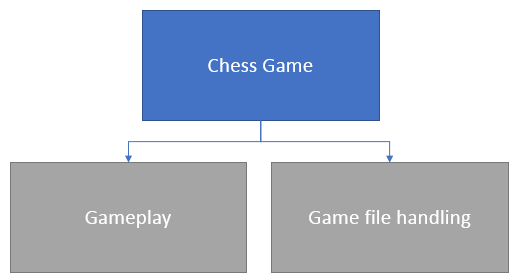
\includegraphics{images/design-charts/top_level}
\end{center}
\subsection{Second Level View}
\begin{center}
	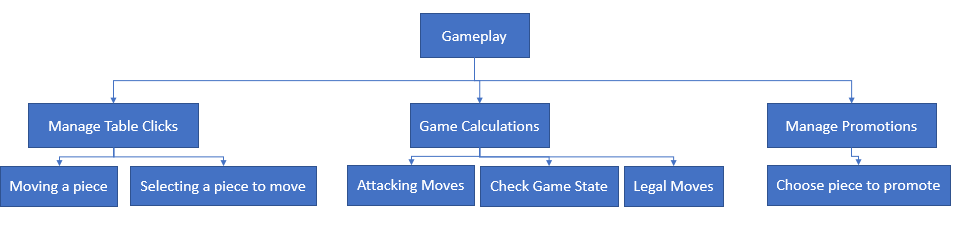
\includegraphics[width=1.0\textwidth]{images/design-charts/gameplay_level}
\end{center}
\begin{center}
	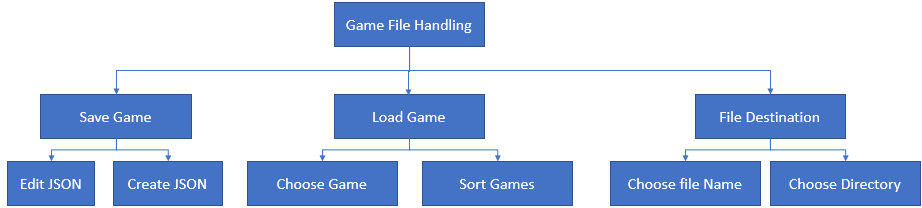
\includegraphics[width=1.0\textwidth]{images/design-charts/filehandling_level}
\end{center}
\section{Class Diagrams}
\begin{center}
	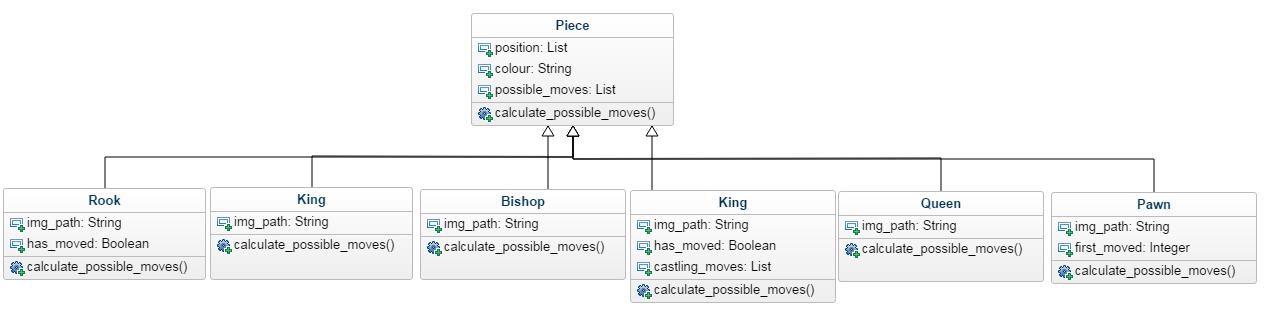
\includegraphics[width=1.0\textwidth]{images/class-diagrams/pieces}
\end{center}
\begin{center}
	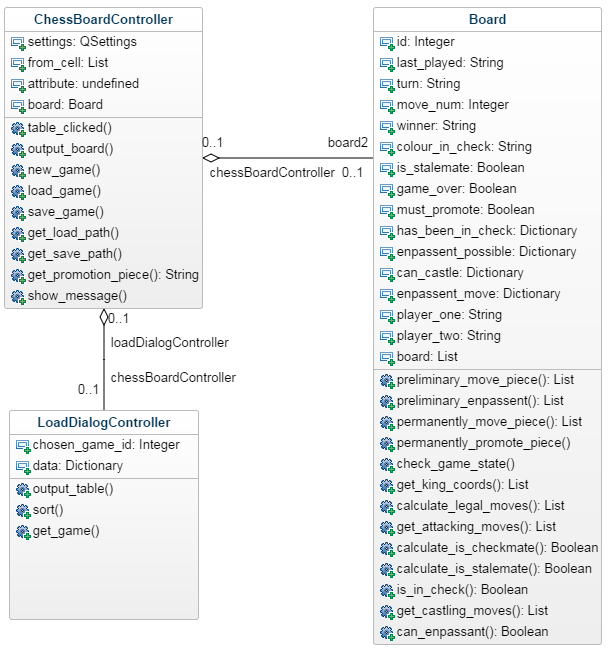
\includegraphics[width=0.9\textwidth]{images/class-diagrams/board}
\end{center}
\subsection{Description of Classes}
\subsubsection{Piece}
The piece class is designed as the base class for which all other types of pieces inherits its attributes from. 

This attribute will be represented by a python list with two elements, where the first element representing the piece's $x$ coordinate and the second element representing its $y$ coordinate. 
\paragraph{colour} This attribute holds a string value of "Black" or "White". This denotes the colour of the piece.
\paragraph{possible{\_}moves} This attribute is a python list. Each element of the list contains a list of positions denoting all the valid moves the piece can make \textbf{assuming that there are no other pieces on the board}.
\begin{minted}{python}
def calculate_possible_moves(self):
\end{minted}
This function is declared in the piece class and raises a NotImplementedError. This exception is raised so that to make sure that all subclasses of the Piece class implement this method and change it appropriately 
% example of code: \inputminted{python}{../src/pieces.py}

\end{document}          
